\section{The Quantum Measurement Paradox, Scale-Time Calculus, and Nilpotent Collapse}
\label{sec:kuantum_olcum_main}

In standard quantum mechanics, the transition from deterministic Schrödinger evolution ($i\hbar \partial_t \psi = \hat{H}\psi$) to discontinuous, stochastic wavefunction reduction ($|\psi|^2 \to \delta(\mathbf{x} - \mathbf{x}_0)$) remains an unproven postulate (the Copenhagen interpretation). The inability of the von Neumann measurement chain to define a physical boundary, coupled with the fact that measurement is strictly irreversible while the Schrödinger equation is time-reversal symmetric ($t \to -t$), constitutes a longstanding foundational challenge.

In this section, we formulate the quantum measurement problem within Scale-Time Calculus ($\kappa^2 = 0$, Scalor Space, $\mathbb{D}_t$). As we demonstrate: \textbf{The wavefunction does not physically collapse to a single point; rather, an unscaled phase wave across static Euclidean space, when projected onto the coordinate frame of a continuously contracting atomic detector ($\kappa$), creates the geometric appearance of localized collapse.}

\subsection{Scalor Decomposition: Timeless Free Waves vs. Contracting Detectors}
\label{sec:skalor_ayrisimi}

In Scale-Time Algebra, the physical state of a system is defined in Scalor space:
\begin{equation}
    \mathbb{S}(t) = \mathbf{X}_0 + \kappa \cdot \lambda(t), \quad \kappa^2 = 0.
    \label{eq:skalor_durum_olcum}
\end{equation}
Two distinct ontological entities exist:
\begin{enumerate}
    \item \textbf{Free Phase Wave (Photon / Wavefunction $\psi$):} A photon is a transverse elastic phase oscillation in the stationary Euclidean continuum ($\mathcal{E}_\infty$). \textbf{Photons do not contract ($\dot{\lambda} = 0$).} Consequently, their Scalor representation lacks a nilpotent component:
          \begin{equation}
              \mathbb{S}_{\mathrm{wave}} = \mathbf{X}_0 \quad (\kappa = 0 \text{ branch}).
              \label{eq:foton_skalor}
          \end{equation}
          Because physical time satisfies $dt \equiv -\frac{1}{H_0}\frac{d\lambda}{\lambda}$, when $d\lambda = 0$ \textbf{no physical time elapses for a photon ($dt = 0$)}. A free photon is a timeless, uncontracted deterministic phase distribution across static Euclidean space.
    \item \textbf{Observer and Detector (Contracting Matter):} Detectors are composed of atomic vortices undergoing continuous contraction:
          \begin{equation}
              \mathbb{S}_{\mathrm{det}}(t) = \mathbf{X}_{\mathrm{det}} + \kappa \cdot \lambda(t), \quad \dot{\lambda}(t) = -H_0 \lambda(t).
              \label{eq:dedektor_skalor}
          \end{equation}
          Because atomic rulers contract monotonically ($d\lambda < 0$), the detector's internal clock advances unidirectionally ($dt > 0$).
\end{enumerate}

\subsection{Nilpotent Scale Projection (\texorpdfstring{$\hat{\mathcal{P}}_\kappa$}{P_kappa}) and the Collapse Appearance}
\label{sec:nilpotent_izdusum}

What the Copenhagen interpretation treats as a discontinuous postulate is, in Scale-Time Calculus, the \textbf{conformal scale projection of an unscaled Euclidean phase onto a contracting reference frame ($\kappa$)}:
\begin{definition}[Nilpotent Measurement Projection]
    \label{def:nilpotent_olcum}
    The interaction between a free wave $\Psi(\mathbf{X}_0)$ in static Euclidean space and a contracting detector $\mathbb{S}_{\mathrm{det}}$ is governed by the nilpotent projection operator $\hat{\mathcal{P}}_\kappa$:
    \begin{equation}
        \hat{\mathcal{P}}_\kappa : \Psi(\mathbf{X}_0) \longrightarrow \psi_{\mathrm{local}}(\mathbf{x}) \ket{\mathbf{x}_0}.
        \label{eq:izdusum_operatoru}
    \end{equation}
\end{definition}

Due to nilpotency ($\kappa^2 \equiv 0$), when an extended phase wave interacts inelastically with a contracting detector atom ($\kappa$), energy exchange is confined to that atom's local boundary:
\begin{equation}
    \hat{\mathcal{P}}_\kappa : \lim_{\mathrm{interaction}} \Delta x_{\mathrm{wave}} \to r_{\mathrm{atom}}(t).
    \label{eq:nilpotent_sonum}
\end{equation}
The extended phase profile is pinned to the detector coordinates, producing a localized particle detection event (\textit{Phase-Pinning}).

\begin{theorem}[Origin of the Apparent Collapse]
    \label{thm:cokus_illuzyonu}
    The wavefunction does not physically collapse to a mathematical point. Because measurement is executed using an atomic length standard that contracts ($\lambda(t) \to 0$), an extended phase wave in Euclidean space is recorded as a localized entity when mapped to the contracting coordinates:
    \begin{equation}
        \lim_{\lambda(t) \to 0} \mathbf{R}_{\mathrm{obs}}(t) = \frac{\mathbf{X}_0}{\lambda(t)} \implies \Delta x_{\mathrm{local}} \to r_{\mathrm{atom}}(t).
        \label{eq:cokus_perspektif}
    \end{equation}
\end{theorem}

\subsection{The Origin of Irreversibility in Quantum Measurement}
\label{sec:geri_donussuzluk_zamani}

Why is quantum measurement irreversible despite the time-reversal symmetry of the Schrödinger equation ($t \to -t$)?
\begin{enumerate}
    \item Physical time elapses ($dt > 0$) as a consequence of matter contraction ($\dot{\lambda} < 0$).
    \item A photon propagating through the quiescent vacuum does not contract, remaining timeless ($dt_{\mathrm{photon}} = 0$).
    \item When a contracting detector atom absorbs the photon's phase, the wavefront is locked into that atom's internal contraction log ($dt > 0$).
    \item Because atomic scale contraction is monotonic ($\dot{\lambda} < 0$), the measurement record cannot be reversed in time.
\end{enumerate}

\begin{figure}[h!]
    \centering
    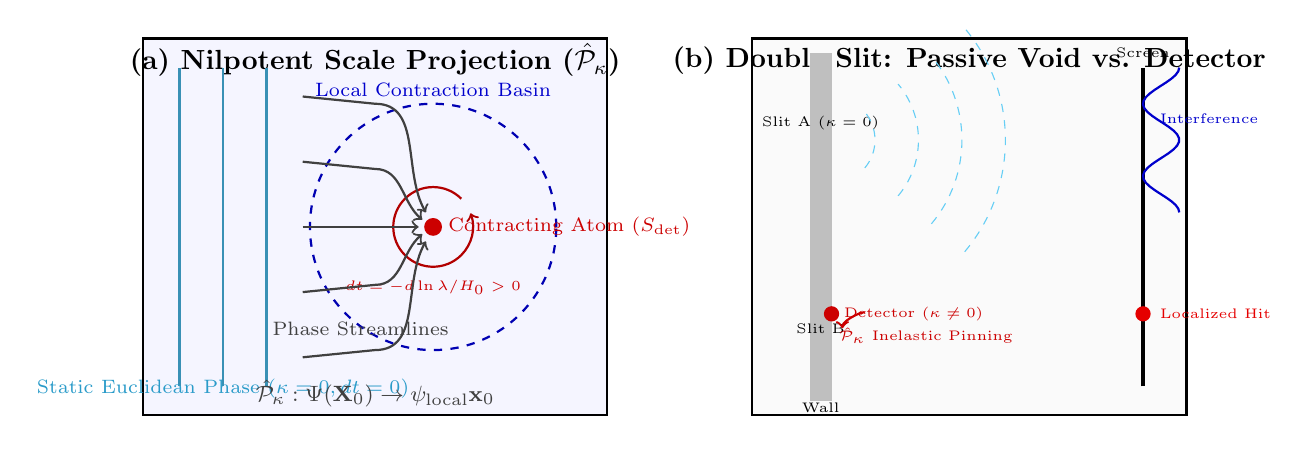
\begin{tikzpicture}[scale=0.92]
        % Panel A: Scale Projection
        \begin{scope}[shift={(-4.4,0)}]
            \draw[thick, fill=blue!4] (-3.2,-2.6) rectangle (3.2,2.6);
            \node at (0, 2.3) {\textbf{(a) Nilpotent Scale Projection ($\hat{\mathcal{P}}_\kappa$)}};

            % Static plane waves in E_infinity
            \foreach \x in {-2.7, -2.1, -1.5} {
                    \draw[cyan!70!black, thick] (\x, -2.2) -- (\x, 2.2);
                }
            \node[cyan!80!black, above] at (-2.1, -2.5) {\scriptsize Static Euclidean Phase ($\kappa=0, dt=0$)};

            % Resonant cross section boundary
            \draw[dashed, blue!70!black, thick] (0.8,0) circle (1.7);
            \node[blue!80!black] at (0.8, 1.9) {\scriptsize Local Contraction Basin};

            % Atom vortex sink
            \fill[red!80!black] (0.8,0) circle (3.5pt) node[right=2pt] {\scriptsize Contracting Atom ($\mathbb{S}_{\mathrm{det}}$)};
            \draw[red!70!black, thick, ->] (0.8,0) ++(45:0.55) arc (45:380:0.55);
            \node[red!80!black, below] at (0.8, -0.6) {\tiny $dt = -d\ln\lambda/H_0 > 0$};

            % Streamlines converging to atom
            \draw[thick, darkgray, ->] (-1.0, 1.8) -- (0.0, 1.7) to[out=0, in=120] (0.7, 0.2);
            \draw[thick, darkgray, ->] (-1.0, 0.9) -- (0.0, 0.8) to[out=0, in=140] (0.65, 0.1);
            \draw[thick, darkgray, ->] (-1.0, 0.0) -- (0.6, 0.0);
            \draw[thick, darkgray, ->] (-1.0, -0.9) -- (0.0, -0.8) to[out=0, in=-140] (0.65, -0.1);
            \draw[thick, darkgray, ->] (-1.0, -1.8) -- (0.0, -1.7) to[out=0, in=-120] (0.7, -0.2);
            \node[darkgray] at (-0.2, -1.4) {\scriptsize Phase Streamlines};
            \node[darkgray] at (0, -2.3) {\footnotesize $\hat{\mathcal{P}}_\kappa : \Psi(\mathbf{X}_0) \to \psi_{\mathrm{local}} \ket{\mathbf{x}_0}$};
        \end{scope}

        % Panel B: Double Slit
        \begin{scope}[shift={(3.8,0)}]
            \draw[thick, fill=gray!4] (-3.0,-2.6) rectangle (3.0,2.6);
            \node at (0, 2.3) {\textbf{(b) Double Slit: Passive Void vs. Detector}};

            % Barrier with two slits
            \fill[gray!50] (-2.2, 1.1) rectangle (-1.9, 2.4);
            \fill[gray!50] (-2.2, -1.1) rectangle (-1.9, 1.1);
            \fill[gray!50] (-2.2, -2.4) rectangle (-1.9, -1.1);
            \node at (-2.05, -2.5) {\tiny Wall};

            % Slit A: Pure vacuum, elastic propagation
            \node[above] at (-2.05, 1.2) {\tiny Slit A ($\kappa=0$)};
            \foreach \r in {0.6, 1.2, 1.8, 2.4} {
                    \draw[cyan!60, dashed] (-1.9, 1.2) ++(-40:\r) arc (-40:40:\r);
                }

            % Slit B: Detector with inelastic absorption
            \node[below] at (-2.05, -1.2) {\tiny Slit B};
            \fill[red!80!black] (-1.9, -1.2) circle (3pt) node[right=1pt] {\tiny Detector ($\kappa \neq 0$)};
            \draw[red!80!black, thick, ->] (-1.5, -1.2) to[out=30, in=90] (-1.75, -1.4);
            \node[red!80!black] at (-0.6, -1.5) {\tiny $\hat{\mathcal{P}}_\kappa$ Inelastic Pinning};

            % Detection Screen
            \draw[very thick, black] (2.4, -2.2) -- (2.4, 2.2);
            \node[above] at (2.4, 2.2) {\tiny Screen};

            % Localized spot vs fringe
            \draw[thick, blue!80!black, domain=-1.0:1.0, samples=40] plot ({2.4 + 0.5*(cos(\x*180)^2)}, {\x + 1.2});
            \node[blue!80!black, right] at (2.5, 1.5) {\tiny Interference};
            \fill[red!90!black] (2.4, -1.2) circle (3pt);
            \node[red!90!black, right] at (2.5, -1.2) {\tiny Localized Hit};
        \end{scope}
    \end{tikzpicture}
    \caption{\textbf{(a)} Nilpotent projection ($\hat{\mathcal{P}}_\kappa$) of a timeless Euclidean phase wave ($\kappa=0$) onto a contracting detector frame. \textbf{(b)} In the double-slit experiment, passive openings act as elastic Euclidean vacuum voids ($\kappa=0$) preserving phase coherence, whereas an active detector performs an inelastic $\kappa$-projection, pinning the wave to a local center (\textit{phase-pinning}).}
    \label{fig:skalor_olcum_cift_yarik}
\end{figure}

\subsection{Double-Slit Experiment: Passive Barrier vs. Active Detector}
\label{sec:cift_yarik_cozum}

Why does the barrier wall not destroy interference, while an active detector at the slit does?
\begin{enumerate}
    \item \textbf{Passive Wall and Slits (Elastic Boundary):} Atoms bordering the slits are off-resonance ($\Delta E = 0$). The open slits contain \textbf{pure Euclidean vacuum ($\kappa = 0$)}. Wavefronts traverse the geometry elastically, preserving mutual coherence and producing standard interference fringes:
          \begin{equation}
              I(\theta) = 4 I_0 \cos^2\left( \frac{\pi d \sin\theta}{\lambda} \right).
              \label{eq:girisim_sacagi_main}
          \end{equation}
    \item \textbf{Active Detector at a Slit (Inelastic $\kappa$-Projection):} Detecting which slit the photon passed through requires an inelastic energy transfer ($\hbar\omega$). Once the phase is transferred to the detector's internal degrees of freedom ($\hat{\mathcal{P}}_\kappa$), phase coherence with the alternate path is extinguished, replacing interference fringes with classical intensity summation:
          \begin{equation}
              I_{\mathrm{total}} = I_1 + I_2.
              \label{eq:klasik_toplam}
          \end{equation}
\end{enumerate}

\subsection{Bell Non-Locality and the Undivided Vacuum Continuum}
\label{sec:bell_ve_nonlokalite}

This formulation does not invoke local hidden variables. The quiescent Euclidean vacuum $\mathcal{E}_\infty$ is a continuous, indivisible manifold. Entangled photons share an unbroken phase continuity regardless of spatial separation. The violation of Bell inequalities (confirmed by Clauser, Aspect, and Zeilinger) reflects the holistic continuity of the stationary background rather than superluminal signaling.
